\documentclass[../main-manifolds.tex]{subfiles}

\begin{document}
\providecommand{\szz}{\mathcal{S}}
\providecommand{\ccinf}{C_c^\infty}

% Topologies
\providecommand{\Taux}{\Tau_\xx}
\providecommand{\Tauy}{\Tau_\yy}
\providecommand{\Tauxy}{\Tau_{\xx\times\yy}}

% Basis
\providecommand{\Bx}{\borel_\xx}
\providecommand{\By}{\borel_\yy}
\providecommand{\Bxy}{\borel_{\xx\times\yy}}


\fchapter{A: Review of Topology}
\begin{wts}[Folland Theorem 4.14]
    Suppose that $A$ and $B$ are disjoint closed subsets of the normal space $X$, and let $\Delta = \{k2^{-n}: n\geq 1 \text{ and } 0<k<2^n\}$ be the set of dyadic rationals in $(0,1)$. There is a family $\{U_r:r\in\Delta\}$ of open sets such that
    \begin{enumerate}
        \item $A\subseteq U_r\subseteq B^c$ for every $r\in \Delta$,
        \item $\overline{U_r}\subseteq U_s$ for $r<s$, and
        \item For every $r<s$, $\cl{U}_r\subseteq U_s$
    \end{enumerate}
\end{wts}
\newcommand{\ksmall}{(k-1)/2^N}
\newcommand{\kbig}{(k+1)/2^N}
\newcommand{\jiggle}[1]{\mathcal{J}({#1})}
\begin{proof}
    The goal of this proof is to show that for every $r\in \Delta$, there exists a open $U_r$ that satisfies the above. As usual for these types of proofs we will proceed by induction. We can divide the problem by 'layers' (as I will hereinafter explain).\\
    
    Let us suppose that for some $N\geq 1$ that all previous $U_r$ in previous layers have been constructed properly, meaning if $r = k/2^n$, then for every $1\leq n \leq N-1$, we have
    \[
    r = \dfrac{k}{2^n},\:1\leq n\leq N-1,\: 1\leq k\leq 2^{n-1}
    \]
    And by 'constructed properly', we mean that for each $U_r$,
    \begin{itemize}
        \item $A\subseteq U_r\subseteq B^c$ and 
        \item $U_r\in \Tau_X$
    \end{itemize}
    Then for this fixed layer $N\geq 1$, we only have to construct the $U_{k/2^N}$ for every odd $k$, this is because if $k$ is an even number, then $k=2j$ and $r = 2j/2^N = j/2^{N-1}$ and for this particular $U_r$ is already constructed. So for every odd $k = 2j+1$, the sets of the form $U_{(k-1)/2^N}$ and $U_{(k+1)/2^N}$ are already defined, and satisfy
    \[
    A\subseteq \cl{U}_{\ksmall}\subseteq U_{\kbig}\subseteq B^c
    \]
    For every $k-1\neq 0$ and $k+1\neq 1$. (We will consider these cases later). We claim that for every pair of open sets, $E_1, E_2\in\Tau_X$, then there exists some open set $G\in\Tau_X$ such that if $(E_1,E_2)\in H\subseteq (\Tau_X\times\Tau_X)$ where $H$ is defined as the set
    \[
    H = \left\{(E_1,E_2)\subseteq(\Tau_X\times\Tau_X): \cl{E_1}\cap E_2^c=\varnothing\right\}
    \]
    Then there exists some $G=\jiggle{E_1,E_2}\in\Tau_X$ such that
    \[
    E_1\subseteq\cl{E_1}\subseteq G\subseteq \cl{G}\subseteq E_2
    \]
    Now consider any any $(E_1,E_2)\in H$, then this pair induces a pair of disjoint sets $\cl{E_1}$ and $E_2^c$ since 
    \[
    \cl{E_1}\subseteq E_2\implies\cl{E_1}\cap E_2^c=\varnothing
    \]
    And by normality, there exists disjoint open sets $G_1$, $G_2$ such that
    \begin{itemize}
        \item $\cl{E_1}\subseteq G_1\in \Tau_X$
        \item $E_2^c\subseteq G_2\in\Tau_X$
        \item $G_1\cap G_2=\varnothing\implies G_1\subseteq G_2^c\subseteq E_2$
        \item Since $G_2^c$ is a closed set that contains $G_1$ as a subset, $\cl{G_1}\subseteq G_2^c\subseteq E_2$
    \end{itemize}
    It is at this point that we will make no further mention of $G_2$ (so we may discard the notion of $G_2$ in our minds). Let us now replace $G$ with $G_1$ then it is an easy task to verify that $G=G_1=\jiggle{E_1,E_2}$ has the required properties.\\
    
    Now define for every odd $k$, since $(U_{\ksmall},U_{\kbig})\in H$ (we note in passing that $\mathcal{J}$ is not a function as the set $G$ may not be unique).
    \[
    U_{k/2^N} = \mathcal{J}\left(U_{\ksmall},U_{\kbig}\right)
    \]
    Then, if $U_{\ksmall}$ and $U_{\kbig}$ is 'well constructed' we have
    \[
    A\subseteq\cl{U}_{\ksmall}\subseteq U_{\kbig}\subseteq B^c
    \]
    Therefore $U_{k/2^N} = \jiggle{U_{\ksmall},U_{\kbig}}$ sits 'right inbetween' the two sets so that
    \begin{itemize}
        \item $A\subseteq \cl{U}_{\ksmall}\subseteq U_{k/2^N}$ and
        \item $\cl{U}_{k/2^N}\subseteq U_{\kbig}\subseteq B^c$
    \end{itemize}
    Combining the above two estimates will give us a 'well constructed' $U_{k/2^N}$ for every $k-1\neq 0$ and $k+1\neq 1$. Now let us deal with the remaining pathological cases.\\
    
    If $k-1$ so happens to be $0$, then no $r\in\Delta$ satisfies $r = 0/2^N$, and we substitute 
    \[
    \cl{U}_0 = A,\quad \text{ or alternatively, } U_0 = A^o
    \]
    Then $U_0\in\Tau_X$, $\cl{U}_0=A\subseteq B^c$. It is at this point that we must mention that $0,1 \notin \Delta$, so $U_0$ and $U_1$ do not have to obey the rules we have laid out for $U_{r\in\Delta}$.\\
    
    Now if $k+1$ is equal to $2^N$ (this makes $r = (k+1)/2^N = 1$) we define
    \[
    U_1=B^c\in\Tau_X
    \]
    With this, for every $0\leq m \leq 2^N -1, U_{m/2^N}$ must staisfy 
    \[
    \cl{U}_{m/2^N}\subseteq B^c = U_1
    \]
    And the pair $(U_{\ksmall},U_{\kbig})\in H$ (even for when $N=1$, since $A = \cl{U}_0\subseteq U_1 = B^c$) and a corresponding $U_{k/2^N} = \jiggle{\cdot,\cdot}$ such that 
    \begin{itemize}
        \item $A\subseteq \cl{U}_{\ksmall}\subseteq U_{k/2^N}$
        \item $\cl{U}_{\kbig}\subseteq B^c$
    \end{itemize}
    Now as a final step, we complete the base case for when $N=1$. We would only have to construct for $k=1$, since 
    \[
    U_{1/2} = \jiggle{U_0,U_1} = \jiggle{A,B^c}
    \]
    Apply the induction step, and the proof is complete, at long last.
\end{proof}

\begin{wts}[Folland Theorem 4.15: Urysohn's Lemma]
Urysohn's Lemma. Let $X$ be a normal space, if $A$ and $B$ are disjoint closed subsets of $X$, then there exists a $f\in C(X,[0,1])$ such that $f=0$ on $A$ and $f=1$ on $B$.
\end{wts}
\begin{proof}
Let $r\in \Delta$ be as in Lemma 4.14, and set $U_r$ accordingly except for $U_1=X$. Define 
\[
f(x) = \inf\{k:x\in U_k\}
\]
Let us also write $W=\{k:x\in U_k\}$, Then for every $x\in A$ we have $f(x)=0$, since by the construction of the 'onion' function in Lemma 4.14, for each $r\in \Delta\cap(0,1)$, 
\[
x\in A\subseteq U_r\implies f(x)\leq r
\]
Since $r>0$ is arbitrary, and $0\in W$, we can use a classic $\varepsilon$ argument. If $f(x)>0$ then there exists some $0<r<f(x)$ by density of the dyadic rationals on the line, if $f(x)<0$ then this implies that there exists some $f(x)<r<0$ such that $x\in U_r$, but no $r\in \Delta$ can be negative, hence $f(x)=0$.\\

Now, for every $x\in B$, since $A$ and $B$ are disjoint, and $A\subseteq U_r\subseteq B^c$, then for every $x\in B$ means that $x$ is not a member of any $U_r$, but we set $U_1=X$. Since none of the $r\in(0,1)$ is a member of the set we are taking the infimum, and $x\in U_1=X$. The $\varepsilon$ argument follows: suppose for every $\varepsilon>0$, $(1-\varepsilon)\notin W$, and $1\in W$, then $f(x)=1$.\\

Since $x\in U_1=X$, for every $x\in X$, $f(x)\leq 1$, and $f(x)$ cannnot be negative as $r>0$ for every $r\in \Delta$. So $0\leq f(x)\leq 1$. Now we have to show that this $f(x)$ is continuous. The remainder of the proof is divided into two parts. We would like to show that the inverse images of the half lines are open in $X$. So $f^{-1}((-\infty,\alpha))\in \mathcal{T}$ and $f^{-1}((\alpha,+\infty))\in\mathcal{T}$.\\

Suppose that $f(x)<\alpha$, so $\inf W<\alpha$, and using the density of $\Delta$, there exists an $r$, $f(x)<r<\alpha$ such that $x\in U_r$ such that $x\in \bigcup_{r<\alpha}U_r$. So $f^{-1}((-\infty,\alpha))\subseteq \bigcup_{r<\alpha}U_r$.\\

Fix an element $x\in\bigcup_{r<\alpha}U_r$, this induces an $r$ such that $\inf W\leq r<\alpha$ therefore $f(x)<\alpha$, and $\bigcup_{r<\alpha}U_r\subseteq f^{-1}((-\infty,\alpha))$.

For the second case, suppose that $f(x)>\alpha$, then $\inf W>\alpha$, and there exists an $r$ (by density) such that $\inf W>r>\alpha$ such that for every $k\in W$, $k\neq r$. Therefore $x\notin U_r$, but by density again, and using the property of the onion function: for every $s<r$ we get $\overline{U_s}\subseteq U_r$, taking complements (which reverses the estimate) — we have $x\notin \overline{U_s}$, but $\left(\overline{U_s}\right)^c$ is open in $X$. It immediately follows that
\[
x\in f^{-1}((\alpha,+\infty))\implies x\in (U_r)^c\subseteq \left(\overline{U_s}\right)^c\subseteq\bigcup_{s>\alpha}\left(\overline{U_s}\right)^c
\]
So $f^{-1}((\alpha,+\infty))$ is a subset of $\bigcup_{s>\alpha}\left(\overline{U_s}\right)^c$. To show the reverse, fix an element $x$ in the union, then this induces some $x\in \left(\overline{U_s}\right)^c\subseteq (U_s)^c$. Then for this $s>\alpha$, $(-\infty,s)$ contains no elements of $W$. This is because for every $p<s$ implies that $(U_s)^c\subseteq(U_p)^c$, so $p\notin W$. Our chosen $s$ is a lower bound for $W$, and $\alpha<s\leq\inf W =f(x)$.\\

Since all of the inverse images from the generating set of $(\mathbb{R},\mathcal{T}_{\mathbb{R}})$ are open in $X$, using Theorem 4.9 finishes the proof.
\end{proof}

Notes on the construction of the countable 'onion' sequence within a normal space $\xx$.\\

If $\xx$ is a normal space, and $A$ and $B$ are disjoint closed subsets, then we can easily find an open $U$ with
\begin{equation}\label{eq:UrysohnLemma-Seashells}
    A\subseteq U \subseteq \cl{U}\subseteq B^c
\end{equation}
We say that $U$ hides in $B^c$ if the closure of $U$ is contained in $B^c$. Define $\Delta_n = \bigset{k2^{-n},\: 1 < k < 2^{n}}$, so that $\Delta_n\subseteq(0,1)$ for all $n\geq 1$. Notice 
\[
    \Delta_1\supseteq \cdots\supseteq \Delta_n\supseteq \Delta_{n+1}
\]
and the even indices for $\Delta_{n+1}$ are contained in $\Delta_n$. Suppose $\Delta_n$ is well defined, it suffices to choose the odd indices for $\Delta_{n+1}$. If $r = j2^{-(n+1)}$, where $j$ is odd, then $r$ sits in between precisely two elements in $\Delta_n\cup\{0,1\}$. If $r$ sits between an endpoint, then define $\cl{U_0} = A$, and $B^c = U_1$. And denote the closest left and neighbours by $s$, $t$ respectively. If $s<r<t$, it is clear that $\cl{U_s}$ and $U_t^c$ are disjoint closed sets.\\

Use the 'normal space' construction to obtain an superset of $\cl{U_s}$ that hides in $U_t$, denote this open set by $U_r$, and similar to \Cref{eq:UrysohnLemma-Seashells}
\[
    \cl{U_s}\subseteq U_r\subseteq \cl{U_r}\subseteq U_t
\]
Now that the construction of this sequence is complete, we wish to prove Urysohn's Lemma. Let $A$ and $B$ be disjoint closed sets. And define 
\[
    f(x) = \inf\bigset{r\in\Delta\cup\{1\},\: x\in U_r}
\]
where $U_1 = \xx$. So that $0\leq f(x)\leq 1$ is immediate. If $x\in A$, then $x$ is in all $U_r$, and by density of $\Delta\subseteq(0,1)$, we have $f(x)=0$. Conversely, if $x\in B$ then $x\notin U_r$ for all $r\in\Delta$, if $E$ denotes the indices in $\Delta$ where $x\in U_s$ when $s\in E$,
\begin{equation}\label{inequality shortcut infimum intervals}
    (-\infty,\: r)\subseteq E^c\iff E\subseteq [r,\: +\infty)\iff\inf(E)\geq r
\end{equation}
Send $r\to 1$ and $f(x) = 1$. Thus $f|_{A}=0$ and $f|_{B}=1$.\\

To show continuity, it suffices to show that the inverse images of the open half $\bigset{(x > \alpha),\: (x < \alpha)}_{\alpha\in\real}$ lines are indeed open in $\xx$. Let $\alpha$ be fixed. And if $x\in \{f<\alpha\}$, we can 'wiggle' the infimum towards the right (towards $\alpha$), and using density of $\Delta$ within $(0,1)$, there exists a $r\in E$ that satisfies $f(x) < r < \alpha$. This is equivalent to 
\[
    x\in \bigcup_{r<\alpha} U_r
\]
If there exists an $r<\alpha$ st $x$ belongs to $U_r$ as an element, then $f(x)\leq r < \alpha$.\\

If $f(x) > \alpha$, then $(-\infty,\: \alpha)\subseteq E^c$, by  \Cref{inequality shortcut infimum intervals}. Suppose $\alpha<1$, otherwise $\{f>\alpha\}=\varnothing$. Wiggle $f(x)$ to the left and obtain an $r\in\Delta$, $\alpha<r<f(x)$ with $x\notin U_r$. By density again, take any $s<r$ by a small amount (st $s>\alpha$, $s\in \Delta$), and
\[
    \cl{U}_s\subseteq U_r\iff U_r^c\subseteq\cl{U}_s
\]
so that $x\in \cl{U}_s^c$ for some $s>\alpha$. This is equivalent to 
\[
    x\in\bigcup_{s>\alpha}\cl{U}_s^c
\]
Conversely, if $x\notin \cl{U}_s^c$ for some $s>\alpha$,  since $\{U_r\}$ (thus $\{\cl{U}_r\}$) is increasing, and $x\notin U_r$ for every $r\leq s$. Hence,
\[
    (-\infty,\: s]\subseteq E^c\iff E\subseteq (s,\: +\infty)\iff f(x)\geq s>\alpha
\]


\newpage
\topheader{Compactness}
Compactness is one of the most important concepts in topology and analysis.

\begin{definition}[Compact topological space]\label{chp4:compact-space-definition}
    A topological space $\xx$ is compact if every open covering $\{U_\alpha\}$ contains a finite subcover. That is, if $\{U_\alpha\}$ is an arbitrary collection of open sets, then
    \[
        \xx  = \bigcup U_{\alpha\in A}\implies\bigcup_{j\leq n}U_{\alpha_j}
    \]
\end{definition}

\begin{definition}[Compact set]\label{chp4:compact-set-definition}
    $E\subseteq\xx$ is compact if it is compact in the subspace topology.
\end{definition}

\begin{definition}[Precompact set]\label{chp4:precompact-set-definition}
    $E\subseteq\xx$ is precompact if its closure is compact (as a subset).
\end{definition}

\begin{definition}[Paracompact space]\label{chp4:paracompact-set-definition}
    A topological space $\xx$ is paracompact if every open covering of $\xx$ has a locally finite open refinement that covers $\xx$.
\end{definition}

\begin{definition}[Locally finite collection of sets]\label{chp4:locally-finite-definition}
    Let $\acal$ be a collection of subsets of $\xx$. It is called locally finite, if at every point $p\in \xx$, we can find a neighbourhood $U$ of $p$ (not necessarily open), that intersects only finitely many members of $\acal$. In symbols,
    \[
        U\cap E=\varnothing\qq{for all but finitely many}E\in\acal
    \]
    We do not require $\acal$ to be a cover of $\xx$, nor do we require $\acal$ to be a collection of open sets.
\end{definition}

\begin{definition}[Countably locally finite]\label{chp4:countably-locally-finite-definition}
    A collection $\borel$ is countably locally finite if it is the countable union of locally finite families.
    \[
        \borel = \overbracket{\bigcup_{\nat}}^{\mathclap{\substack{\text{countable}\\ \text{union}}}}\borel_n,\quad\text{where each }\borel_n\text{ is a locally finite collection}
    \]
\end{definition}
    
\begin{definition}[Refinement]\label{chp4:refinement-definition}
    If $\acal$ is a collection of sets, $\borel$ is a refinement of $\acal$ if every element $B\in\borel$, induces an element $A\in\acal$, such that $B\subseteq A$.
\end{definition}
\begin{remark}[Intuition for refinements]
    If $\borel$ is a refinement of $\acal$, we can use the 'absolute continuity' muscle. For each element in $\borel$ is dominated by some element (through subset inclusion) in $\acal$. Recall, if $\nu$ and $\mu$ are non-negative measures, then $\nu\ll\mu$ if for every measurable set $E\in\mcal$, $\mu(E)=0\implies \nu(E)=0$.\\
    
    A refinement of a family of sets is another family of sets, whose elements are dominated by some other element in the un-refined family. \emph{Refining families makes them 'smaller', cover less area.}
\end{remark}

\begin{wts}
    Compact Hausdorff spaces are normal, compact subsets of Hausdorff spaces are closed, and closed subsets of compact sets are again compact. 
\end{wts}

\newpage

\topheader{Locally Compact Hausdorff Spaces}
Compactness is an intrinsic topological property (in the subspace topology). We see from Proposition 4.25 that compact Hausdorff spaces are normal, which gives a sufficient condition for us to approximate and extend any continuous function; and allows us to extend certain 'local' properties to 'global' properties. \\

If given a Hausdorff space, not necessarily compact, the natural question is to ask 1) whether a topological space has 'enough' compact subsets to work with, and 2) whether we can embed a given topological space in a larger one to force it to be compact.

\begin{definition}[LCH space]\label{chp4:LCH-definition}
    Let $\xx$ be a Hausdorff space. We call $\xx$ a LCH space if every point $p\in\xx$ admits a compact neighbourhood. That is, a compact set $K$ whose interior contains $p$.
\end{definition} 

We note in passing that the above definition differs slightly from the usual 'local' definitions.

\begin{definition}[Locally connected]\label{chp4:locally-connected-definition}
    Let $\xx$ be a topological space, it is locally connected if for every $x\in\xx$, and open neighbourhood $U$ containing $x$, there exists a connected, open neighbourhood $V$ of $x$ such that $x\in V\subseteq U$.
\end{definition}

\begin{definition}[Locally path-connected]\label{chp4:locally-path-connected-definition}
    Let $\xx$ be a topological space, it is locally connected if for every $x\in\xx$, and open neighbourhood $U$ containing $x$, there exists a path-connected, open neighbourhood $V$ of $x$ such that $x\in V\subseteq U$.
\end{definition}

\begin{definition}[Local homeomorphism]\label{chp4:locally-homeomorphic-definition}
    $\xx$ locally homeomorphic to $\realn$ if every point $x\in\xx$ belongs to a coordinate chart $(U,\phi)$, where $U$ is an open neighbourhood of $x$ and $\phi$ is a homeomorphism from $U\to\phi(U)\subseteq\realn$.
\end{definition}

\begin{definition}[Local diffeomorphism]\label{lee-chp4:local-diffeomorphism-definition}
    Let $M$ be a smooth manifold and $F\in \cinf[M,N]$. $F$ is a local diffeomorphism if every $p\in M$ in its domain induces a neighbourhood $U\subseteq M$ with $F|U:U\to F(U)$ is a diffeomorphism (in the sense of two open sub-manifolds).
\end{definition}



\topheader{Properties of Compact Spaces}
\begin{figure}[htbp]
        \centering
        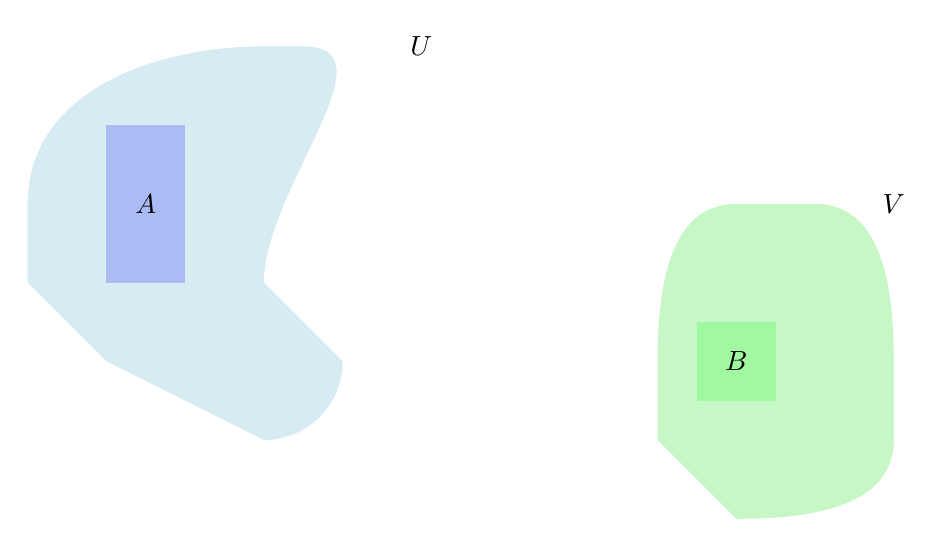
\begin{tikzpicture}
            % Define colors
            \definecolor{lightblue}{RGB}{173,216,230}
            \definecolor{lightgreen}{RGB}{144,238,144}
    
            % Draw the open set U
            \fill[lightblue,opacity=0.5] (1,1) -- (1,2) to[out=90,in=180] (4,4) -- (4.5,4) to[out=0,in=90] (4,1) -- (5,0) to[out=-90,in=0] (4,-1) -- (2,0) -- cycle;
            \node at (6,4) {$U$};
    
            % Draw the closed set A
            \fill[blue,opacity=0.2] (2,1) rectangle (3,3);
            \node at (2.5,2) {$A$};
    
            % Draw the open set V
            \fill[lightgreen,opacity=0.5] (9,-1.2) -- (9,0) to[out=90,in=180] (10,2) -- (11,2) to[out=0,in=90] (12,0) -- (12,-1) to[out=-90,in=0] (10,-2) -- (9,-1) -- cycle;
            \node at (12,2) {$V$};
    
            % Draw the closed set B
            \fill[green,opacity=0.2] (9.5,-0.5) rectangle (10.5,0.5);
            \node at (10,0) {$B$};
        \end{tikzpicture}
        \caption{Closed sets $A$ and $B$ within open sets $U$ and $V$, respectively.}
        \label{lee-appendix-A.45-graphic}
\end{figure}

\begin{wts}\label{lee-appendix-A.45}
Let $\xx$ and $\yy$ be topological spaces.
\begin{enumalpha}
    \item If $F\in C(\xx,\yy)$, and $\xx$ is compact, then $F(\xx)$ is compact.
    \item If $\xx$ is compact and $F\in C(\xx,\real)$, then $F(\xx)$ is bounded, and $F$ attains its supremum and infimum on $\xx$.
    \item A finite union of compact subspaces of $\xx$ is again compact.
    \item If $\xx$ is Hausdorff, and $A$, $B$ are disjoint, compact subspaces of $\xx$, there exists open $U$ and $V$, (see \cref{lee-appendix-A.45-graphic}).
    
    \item Every closed subset of a compact space is compact.
    \item Every compact subset of a Hausdorff space is closed.
    \item Every compact subset of a metric space is bounded.
    \item Every finite product of compact spaces is compact.
    \item Every quotient of a compact space is compact.
\end{enumalpha}
\end{wts}
\newpage
\begin{proof}[Proof of \Cref{lee-appendix-A.45} Part A]
    Let $f\in C(\xx,\yy)$ with $\xx$ compact. Fix an open cover of $f(\xx)$ in the relative topology, 
    \[
        \{U_\alpha\cap f(\xx)\}_{\alpha\in A}\text{ covers }\xx,\: U_\alpha\text{ open in }\yy
    \]    
    So that $\bigcup f^{-1}(U_\alpha) = \bigcup f^{-1}(U_\alpha\cap f(\xx))=\xx$. Since $\{f^{-1}(U_\alpha)\}_{\alpha\in A}$ is an open cover for $\xx$, this induces a finite subcollection of indices $\{\alpha_1,\ldots,\alpha_n\}$ with
    \[
        \bigcup_{j=1}^nf^{-1}(U_{\alpha_j}) = \bigcup_{j=1}^nf^{-1}(U_{\alpha_j}\cap f(\xx))
    \]
    The direct image commutes with unions, therefore
    \[
        f(\xx)=f\biggl(\bigcup_{j=1}^nf^{-1}(U_\alpha\cap f(\xx))\biggr) = \bigcup_{j=1}^nf\biggl(f^{-1}(U_{\alpha_j})\biggr) = \bigcup_{j=1}^n U_{\alpha_j}
    \]
\end{proof}


\begin{proof}[Proof of \Cref{lee-appendix-A.45} Part B]
    Let $\xx$ be compact, and $f\in C(\xx,\real)$, so that $f(\xx)\subseteq\real$ is compact. Compact subsets are closed and bounded in $\real$, let $A = \sup f(\xx)$ and $B = \inf f(\xx)$. Both $A$ and $B$ are accumulation points of $f(\xx)$, so $A = f(x)$ and $B = f(y)$ for some $x$, $y$ in $\xx$.
\end{proof}


\begin{proof}[Proof of \Cref{lee-appendix-A.45} Part C]
    Let $\xx$ be a topological space, and $K_1,\ldots K_n$ be compact subspaces. Denote $K = \bigcup_{j=1}^n K_j$. Let $\{U_\alpha\cap K\}_{\alpha\in A}$ be an open cover for $K$, where $U_\alpha$ is open in $\xx$. We can pass the argument to each individual $K_j$ as follows. Let $1\leq j\leq n$, then $\{U_\alpha\cap K_j\}_{\alpha\in A}$ is an oepn cover for $K_j$, so there exists as finite subcollection of indices $I_j\subseteq A$, (a finite subset of $A$) whose open sets cover $K_j$. Repeat this process for each $j$ and 

    \[
        I = \bigcup_{j=1}^n I_j \text{ is a finite subset of } A
    \]
    with $K_j\subseteq \bigcup_{\alpha\in I_j}(U_\alpha\cap K_j)\subseteq \bigcup_{\alpha\in I_j}(U_\alpha\cap K)$. Taking the union over all $K_j$ reads
    \[
        K = \bigcup_{j=1}^n K_j\subseteq \bigcup_{j=1}^n \bigcup_{\alpha\in I_j}(U_\alpha\cap K)=\bigcup_{\alpha\in I}U_\alpha\cap I
    \]
\end{proof}
\begin{figure}[htbp]
        \centering
        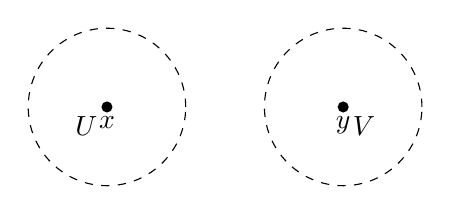
\begin{tikzpicture}
            % Draw the points x and y
            \fill (0,0) circle (2pt) node[below] {$x$};
            \fill (3,0) circle (2pt) node[below] {$y$};
    
            % Draw the open neighbourhoods U and V
            \draw[dashed] (0,0) circle (1) node[below left] {$U$};
            \draw[dashed] (3,0) circle (1) node[below right] {$V$};
        \end{tikzpicture}
        \caption{In a Hausdorff space, any two distinct points $x$ and $y$ can be separated by disjoint open neighbourhoods $U$ and $V$.}
        \label{lee-appendix-A.45D Hausdorff}
    \end{figure}
\begin{proof}[Proof of \Cref{lee-appendix-A.45} Part D]
    Let $\xx$ be Hausdorff. We first prove that compact subspaces of $\xx$ are closed. Indeed, if $K$ is compact in $\xx$, fix any $x\in K^c$. Let $y$ range through the elements of $K$, then $x\neq y$ induces a pair of disjoint open sets $U_y$ and $V_y$, such that
    
\begin{itemize}
    \item $x\in U_y$
    \item $y\in V_y$
    \item $U_y\cap V_y=\varnothing$
    \item See \cref{lee-appendix-A.45D Hausdorff}
\end{itemize}





\begin{figure}[htbp]
    \centering
    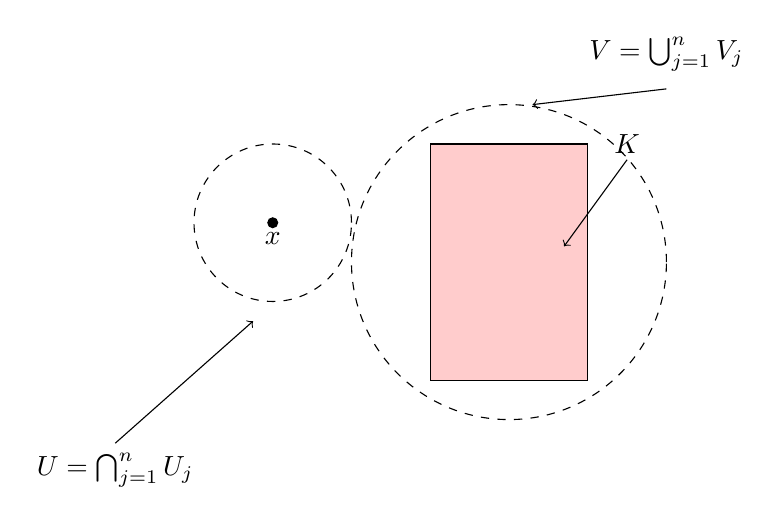
\begin{tikzpicture}
        % Draw the point x in A
        \fill (-0.5,0.5) circle (2pt);
        \node[below] at (-0.5,0.5) {$x$};
        
        % Draw the neighbourhood around x
        \draw[dashed] (-0.5,0.5) circle (1);
        \node[below] at (-2.5,-2.3) {$U=\bigcap_{j=1}^n U_j$};
        \draw[->] (-2.5,-2.3) -- (-0.75,-0.75);

        % Draw the closed set K
        \fill[red,opacity=0.2] (1.5,-1.5) rectangle (3.5,1.5);
        \draw (1.5,-1.5) rectangle (3.5,1.5);
        \node at (4,1.5) {$K$};
        \draw[->] (4,1.3) -- (3.2,0.2);

        % Draw the neighbourhood around K
        \draw[dashed] (2.5,0) circle (2);
        \node[above] at (4.5,2.3) {$V=\bigcup_{j=1}^n V_j$};
        \draw[->] (4.5,2.2) -- (2.8,2);
    \end{tikzpicture}
    \caption{Compact sets are closed in Hausdorff spaces}
    \label{lee-appendix-A.45D-compact-open}
\end{figure}

Let $V_y$ range through all possible $y\in K$, So that $\{V_y\}_{y\in K}$ is an open cover. There exists a finite subcollection of 'anchor points' of $K$, $y_1,\ldots,y_n$ that corresponds with $\{V_{y_j}\}_{j=1}^n$.

A finite intersection of open sets is again open, so 
\[
    U = \bigcap_{j=1}^n U_{y_j}\text{ is open }
\]
Define $V = \bigcup_{j=1}^nV_{y_j}$, so $V\subseteq K$ and $U\cap V = \varnothing$ and $x\in U\subseteq K^c$ (see \cref{lee-appendix-A.45D-compact-open}). Therefore $K$ is closed.\\



\begin{figure}[htbp]
    \centering
    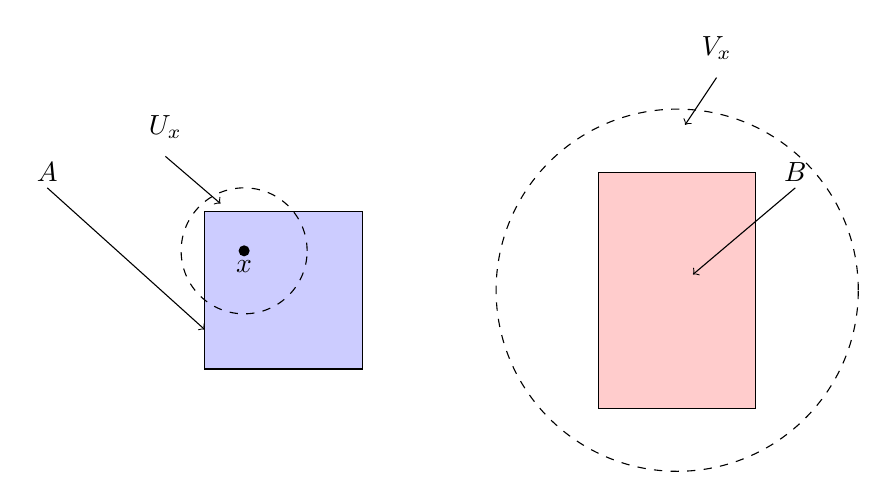
\begin{tikzpicture}
        % Draw the closed sets A and B
        \fill[blue,opacity=0.2] (-1,-1) rectangle (1,1);
        \draw (-1,-1) rectangle (1,1);
        \node at (-3,1.5) {$A$};
        \draw[->] (-3,1.3) -- (-1,-0.5);

        \fill[red,opacity=0.2] (4,-1.5) rectangle (6,1.5);
        \draw (4,-1.5) rectangle (6,1.5);
        \node at (6.5,1.5) {$B$};
        \draw[->] (6.5,1.3) -- (5.2,0.2);

        % Draw the point x in A
        \fill (-0.5,0.5) circle (2pt);
        \node[below] at (-0.5,0.5) {$x$};
        

        % Draw the neighbourhoods around x and B
        \draw[dashed] (-0.5,0.5) circle (0.8);
        \node[above] at (-1.5,1.8) {$U_x$};
        \draw[->] (-1.5,1.7) -- (-0.8,1.1);

        \draw[dashed] (5,0) circle (2.3);
        \node[above] at (5.5,2.8) {$V_x$};
        \draw[->] (5.5,2.7) -- (5.1,2.1);
    \end{tikzpicture}
    \caption{Closed sets $A$ and $B$, point $x$ in $A$, and disjoint neighbourhoods $U$ around $x$ and $V$ around $B$.}
    \label{lee-appendix-A.45D-closed-sets-separation}
\end{figure}

Finally, if $A$ and $B$ are disjoint compact sets, then each $x\in A\subseteq B^c$ induces neighbourhoods $x\in U_x$, and $B\subseteq V_x$ (see \cref{lee-appendix-A.45D-closed-sets-separation}), let $x$ range through all the elements of $A$. By compactness of $A$, this produces a finite subcover, and 

\[
    U = \bigcup_{j=1}^n U_{x_j}\quad V=\bigcap_{j=1}^n V_{x_j}
\]
are disjoint open sets that contain $A$ and $B$ respectively.





\end{proof}

\newpage
%\clearpage

\begin{proof}[Proof of \Cref{lee-appendix-A.45} Part E]
    Let $K\subseteq \xx$ be a closed set of a compact space. Let $\{U_\alpha\cap K\}$ be an open cover for $K$, where each $U_\alpha$ is open in $\xx$. We can append an extra set $K^c$ which is open in $\xx$. The collection

    \[
        W = \{U_\alpha\}\cup \{K^c\} \text{ covers }\xx
    \]
    so there exists a finite subcollection of $W_1,\ldots, W_n$ that cover $\xx$ (since $\xx$ is compact by itself). Remove $K^c$ from this finite subcollection if it exists, and take the intersection with $K$ for each element $W_j$, and

    \[
        \{W_1\cap K,\ldots, W_n\cap K\} = \{U_1\cap K,\ldots, U_n\cap K\}\text{ covers }K
    \]
    so $K$ is compact.
\end{proof}
    
\begin{proof}[Proof of \Cref{lee-appendix-A.45} Part F]
    Proven in Part D.
\end{proof}
    
\begin{proof}[Proof of \Cref{lee-appendix-A.45} Part G]
    let $K\subseteq \xx$ be a compact subset of the metric space $(\xx,d)$. Compact subsets of $\xx$ are totally bounded, and hence bounded.
\end{proof}

\begin{proof}[Proof of \Cref{lee-appendix-A.45} Part H]
    See Tynchonoff's Theorem in Folland Chapter 4.
\end{proof}

\begin{proof}[Proof of \Cref{lee-appendix-A.45} Part I]
    Let $\xx$ and $\yy$ be topological spaces and $\pi: \xx\to\yy$ be a quotient map. So that $\yy$ is endowed with the quotient topology. So that $\pi$ is a surjective continuous map. and $\pi(\xx)=\yy$. Apply Part A, and we see that $\yy$ is compact.
\end{proof}

\end{document}

